\documentclass[12pt,a4paper]{article}

\usepackage[utf8]{inputenc}
\usepackage[T2A]{fontenc}
\usepackage[ukrainian]{babel}
\usepackage{geometry}
\geometry{
    left=2cm,
    right=2cm,
    top=2cm,
    bottom=2cm
}

\usepackage[table]{xcolor}
\usepackage{amsmath}
\usepackage{graphicx}
\usepackage{subcaption}
\usepackage{multirow}
\usepackage{makecell}
\usepackage{pdflscape}
\usepackage{array}
\newcolumntype{C}[1]{>{\centering\arraybackslash}m{#1}}

\usepackage{minted}

\usemintedstyle{vs}
\setminted{linenos, breaklines, frame=single, fontsize=\small}

\RecustomVerbatimCommand{\VerbatimInput}{VerbatimInput}{
    breaklines=true,
    breaksymbolleft={}
}

\usepackage[
  unicode,
  pdftitle={ІО-41, Давидчук А.М., Цифрова схемотехніка, Лабораторна робота №5},
  pdfauthor={Давидчук Артем},
  pdfsubject={Цифрова схемотехніка}
]{hyperref}

\begin{document}

    \hypersetup{pageanchor=false}
    \begin{titlepage}

        \begin{center}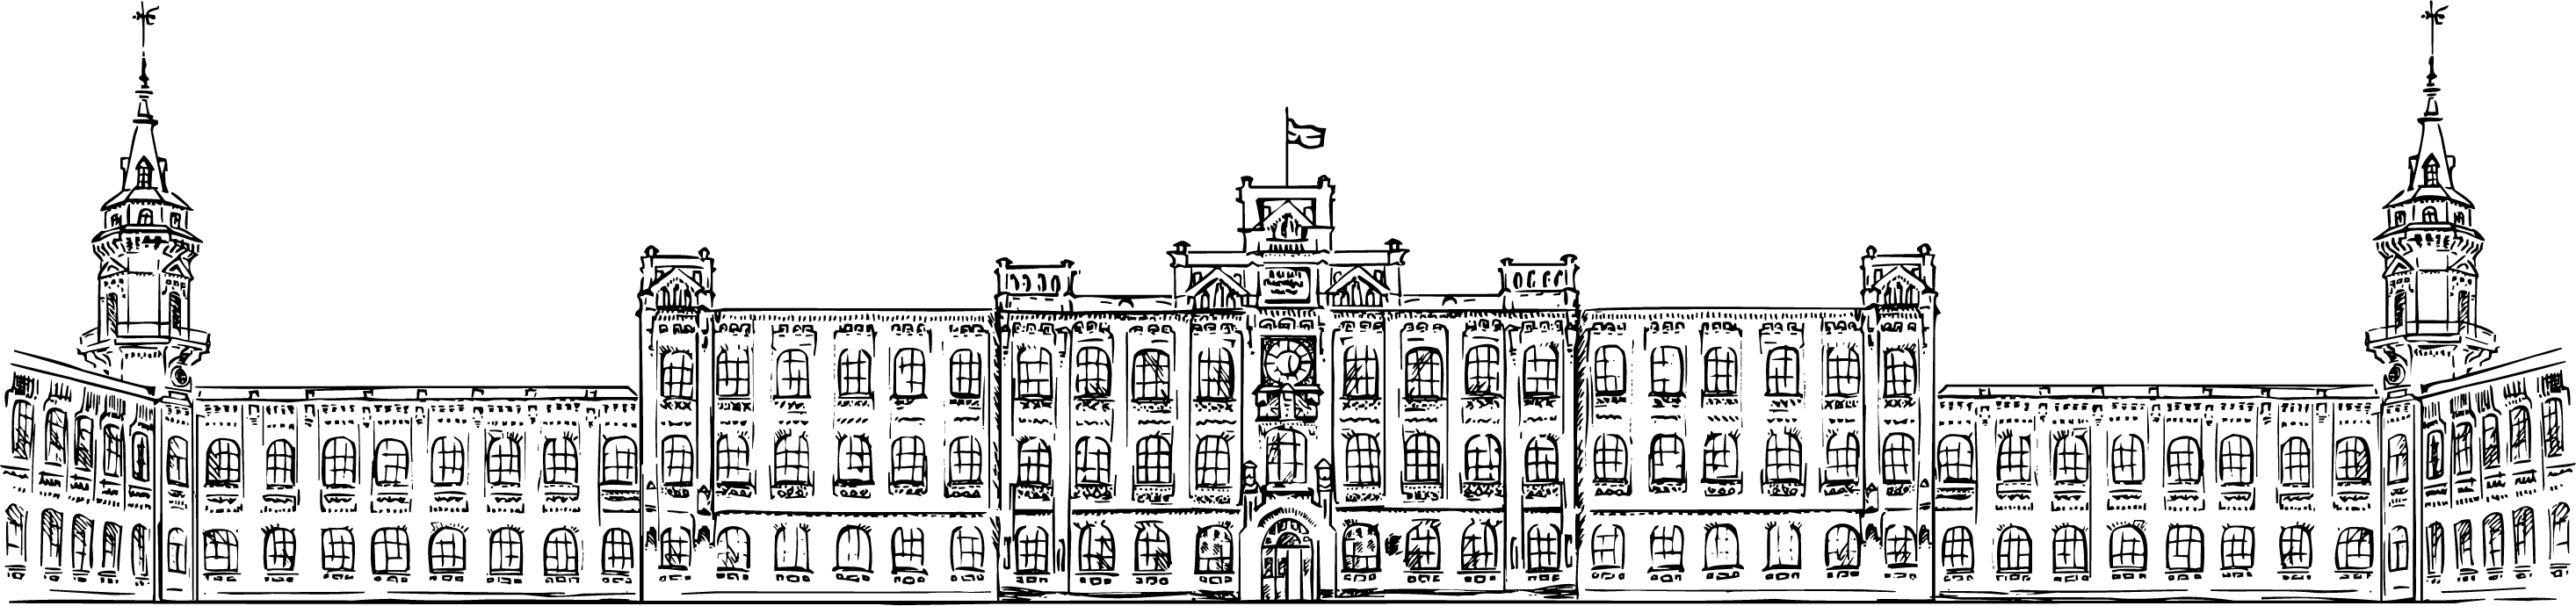
\includegraphics[width=0.7\textwidth]{../../../TITLES/letterhead.png}\end{center}

        \begin{center}
            \large Національний технічний університет України\\
            «Київський політехнічний інститут імені Ігоря Сікорського»\\[1em]
            Факультет інформатики та обчислювальної техніки\\
            Кафедра обчислювальної техніки
        \end{center}

        \vfill

        \begin{center}
            \textbf{\LARGE Цифрова схемотехніка}\\[2em]
            \textbf{\Large Лабораторна робота №5}\\[0.5em]
            «Комбінаційні пристрої. Типові вузли комп'ютера»
        \end{center}

        \vfill

        \begin{flushright}
            Виконав: студент 2 курсу ФІОТ, гр. ІО-41\\
            \textit{Давидчук А. М.}\\
            Залікова книжка № 4106\\[1em]
            Перевірив: \textit{Нікольський С.\,С.}
        \end{flushright}

        \vfill

        \begin{center}Київ --- 2026\end{center}

    \end{titlepage}
    \hypersetup{pageanchor=true}

    \noindent
    \textbf{\underline{Тема:}} «Комбінаційні пристрої. Типові вузли комп'ютера».

    \vspace{1em}

    \begin{center} \textbf{\Large Хід роботи} \end{center}

    Мій номер залікової книжки: 4106, що у двійковому вигляді є 0001 0000 0000 1010.
    Звідси $h_7 = 0, h_6 = 0, h_5 = 0, h_4 = 1, h_3 = 0, h_2 = 1, h_1 = 0$.
    Звідси маю реалізувати дешифратор для семисегментного індикатора:

    \begin{figure}[h]
        \centering
        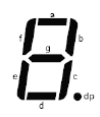
\includegraphics[width=0.2\textwidth]{media/indicator.png}
        \caption{Семисегментний індикатор}
    \end{figure}

    Активний рівень сигналу включення сегмента -- логічний «0». Тобто для засвічення сегмента $a$ на його вході має бути логічний нуль, а для вимкнення певного сегмента -- логічна одиниця. На цій основі побудовано таблицю істинності для функцій $a, b, c, d, e, f, g$ для всіх значень 4-розрядного двійкового числа $x_4x_3x_2x_1$:

    \begin{table}[h]
        \centering
        \renewcommand{\arraystretch}{1.15}
        \begin{tabular}{|cccc|ccccccc|}
        \hline
        $x_4$ & $x_3$ & $x_2$ & $x_1$ & $a$ & $b$ & $c$ & $d$ & $e$ & $f$ & $g$ \\
        \hline
        $0$ & $0$ & $0$ & $0$ & $0$ & $0$ & $0$ & $0$ & $0$ & $0$ & $1$ \\
        $0$ & $0$ & $0$ & $1$ & $1$ & $0$ & $0$ & $1$ & $1$ & $1$ & $1$ \\
        $0$ & $0$ & $1$ & $0$ & $0$ & $0$ & $1$ & $0$ & $0$ & $1$ & $0$ \\
        $0$ & $0$ & $1$ & $1$ & $0$ & $0$ & $0$ & $0$ & $1$ & $1$ & $0$ \\
        $0$ & $1$ & $0$ & $0$ & $1$ & $0$ & $0$ & $1$ & $1$ & $0$ & $0$ \\
        $0$ & $1$ & $0$ & $1$ & $0$ & $1$ & $0$ & $0$ & $1$ & $0$ & $0$ \\
        $0$ & $1$ & $1$ & $0$ & $0$ & $1$ & $0$ & $0$ & $0$ & $0$ & $0$ \\
        $0$ & $1$ & $1$ & $1$ & $0$ & $0$ & $0$ & $1$ & $1$ & $1$ & $1$ \\
        $1$ & $0$ & $0$ & $0$ & $0$ & $0$ & $0$ & $0$ & $0$ & $0$ & $0$ \\
        $1$ & $0$ & $0$ & $1$ & $0$ & $0$ & $0$ & $0$ & $1$ & $0$ & $0$ \\
        $1$ & $0$ & $1$ & $0$ & $0$ & $0$ & $0$ & $1$ & $0$ & $0$ & $0$ \\
        $1$ & $0$ & $1$ & $1$ & $1$ & $1$ & $0$ & $0$ & $0$ & $0$ & $0$ \\
        $1$ & $1$ & $0$ & $0$ & $0$ & $1$ & $1$ & $0$ & $0$ & $0$ & $1$ \\
        $1$ & $1$ & $0$ & $1$ & $1$ & $0$ & $0$ & $0$ & $0$ & $1$ & $0$ \\
        $1$ & $1$ & $1$ & $0$ & $0$ & $1$ & $1$ & $0$ & $0$ & $0$ & $0$ \\
        $1$ & $1$ & $1$ & $1$ & $0$ & $1$ & $1$ & $1$ & $0$ & $0$ & $0$ \\
        \hline
        \end{tabular}
        \caption{\centering Таблиця істинності дешифратора семисегментного індикатора при активному логічному 0}
    \end{table}

    Далі потрібно мінімізувати всі функції $a, b, c, d, e, f, g$ за допомогою діаграм Вейча. Для якісної мінімізації варто розглянути як КНФ, так і ДНФ, а потім обрати форму з найменшою кількістю термів. Результати мінімізації показали, що для функцій $a, b, c, d, e, f$ вигідно взяти МКНФ, а для $g$ -- МДНФ. Відповідні діаграми Вейча:

    \newpage

    \begin{figure}[htbp]
        \centering

        \begin{subfigure}[t]{0.3\textwidth}
            \centering
            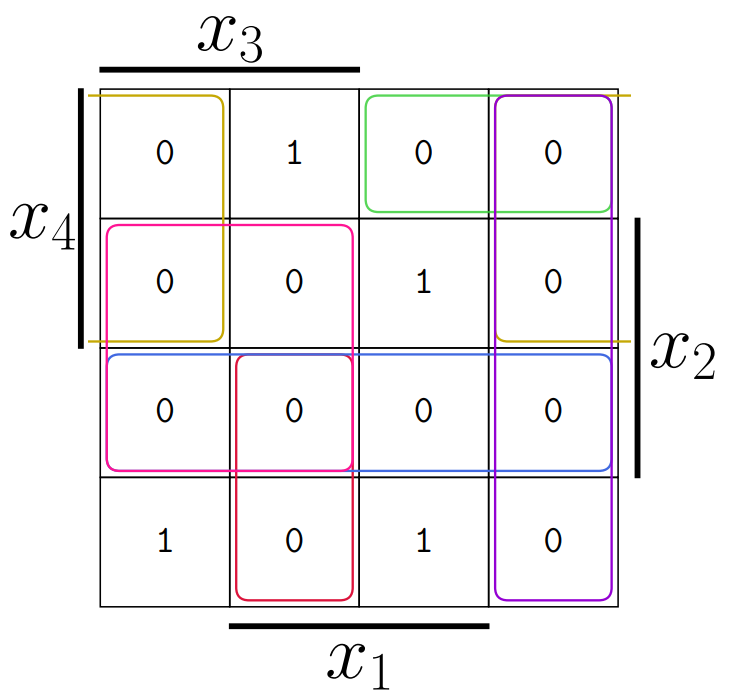
\includegraphics[width=\linewidth]{media/a_veich.png}
            \caption*{\small а) діаграма Вейча сегмента $a$}
        \end{subfigure}
        \hfill
        \begin{subfigure}[t]{0.3\textwidth}
            \centering
            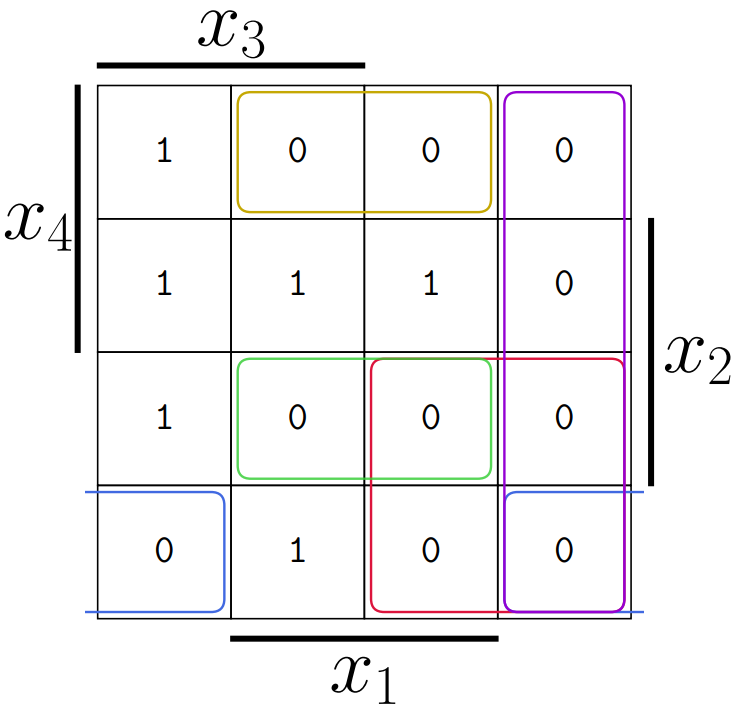
\includegraphics[width=\linewidth]{media/b_veich.png}
            \caption*{\small б) діаграма Вейча сегмента $b$}
        \end{subfigure}
        \hfill
        \begin{subfigure}[t]{0.3\textwidth}
            \centering
            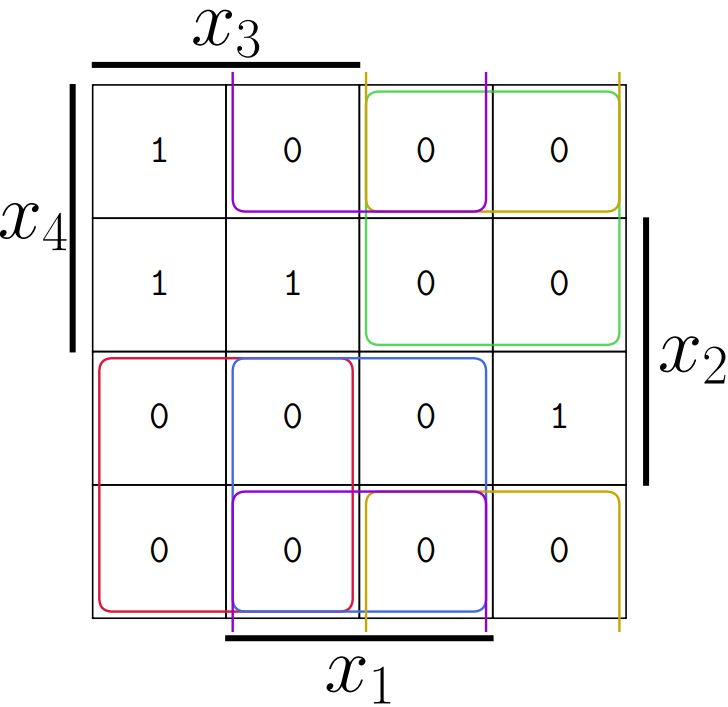
\includegraphics[width=\linewidth]{media/c_veich.png}
            \caption*{\small в) діаграма Вейча сегмента $c$}
        \end{subfigure}

        \vspace{0.8em}

        \begin{subfigure}[t]{0.3\textwidth}
            \centering
            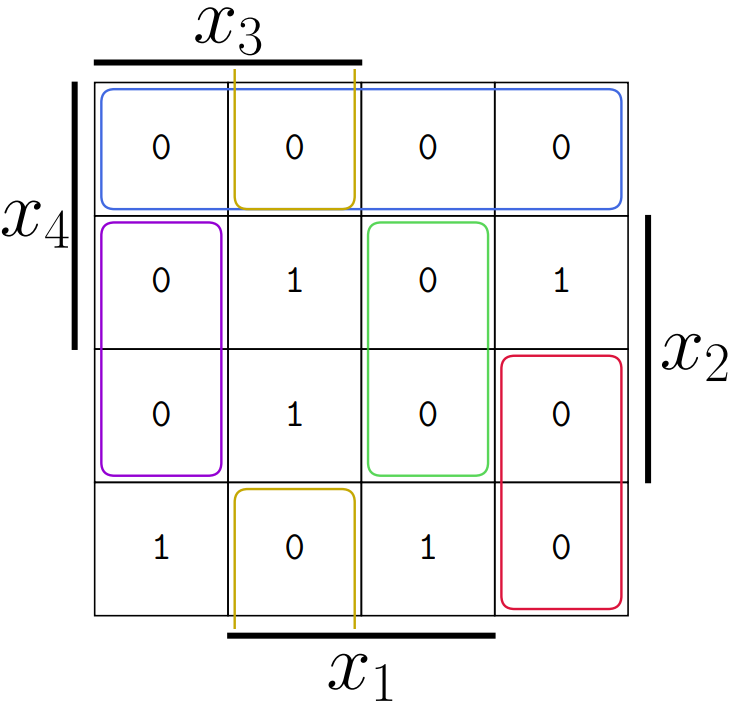
\includegraphics[width=\linewidth]{media/d_veich.png}
            \caption*{\small г) діаграма Вейча сегмента $d$}
        \end{subfigure}
        \hfill
        \begin{subfigure}[t]{0.3\textwidth}
            \centering
            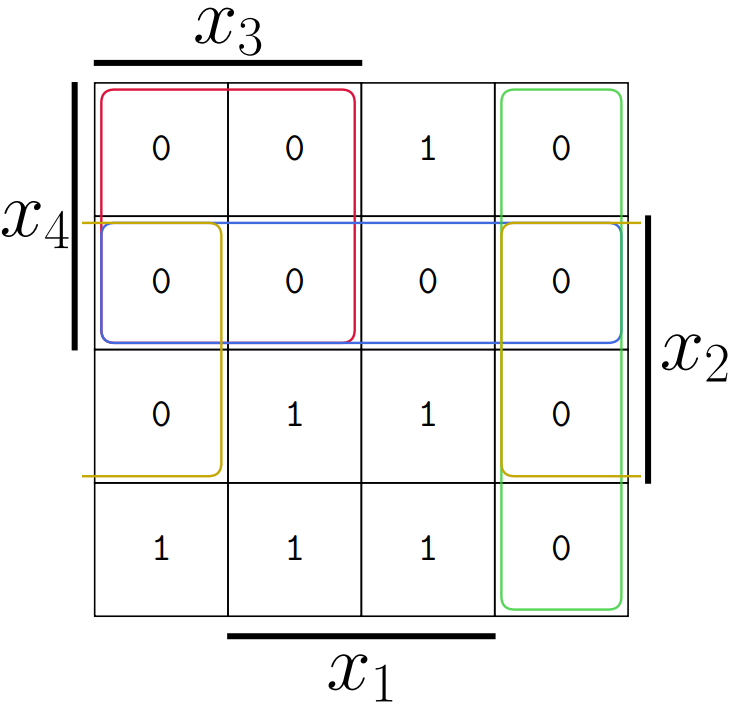
\includegraphics[width=\linewidth]{media/e_veich.png}
            \caption*{\small д) діаграма Вейча сегмента $e$}
        \end{subfigure}
        \hfill
        \begin{subfigure}[t]{0.3\textwidth}
            \centering
            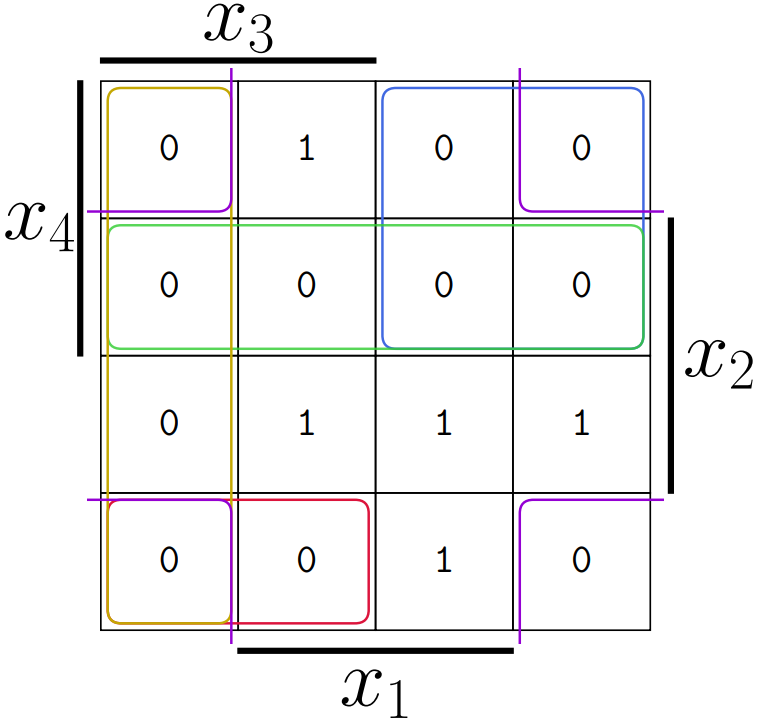
\includegraphics[width=\linewidth]{media/f_veich.png}
            \caption*{\small е) діаграма Вейча сегмента $f$}
        \end{subfigure}

        \vspace{0.8em}

        \begin{subfigure}[t]{0.3\textwidth}
            \centering
            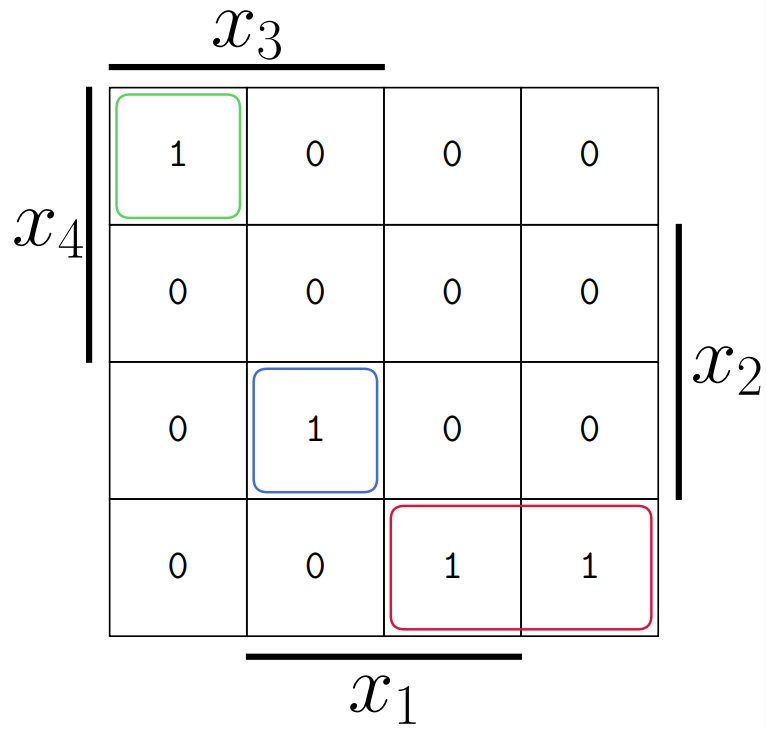
\includegraphics[width=\linewidth]{media/g_veich.png}
            \caption*{\small є) діаграма Вейча сегмента $g$}
        \end{subfigure}

        \caption{\centering Діаграми Вейча для функцій керування сегментами семисегментного індикатора}
    \end{figure}

    \noindent
    Отримані мінімізовані функції мають вигляд:

    \[
    a = (x_4 \vee \overline{x_3} \vee \overline{x_1})
        (x_4 \vee \overline{x_2})
        (\overline{x_4} \vee x_3 \vee x_2)
        (\overline{x_4} \vee x_1)
        (x_3 \vee x_1)
        (\overline{x_3} \vee \overline{x_2})
    \]

    \[
    b = (x_4 \vee x_3)
        (x_4 \vee x_2 \vee x_1)
        (x_4 \vee \overline{x_2} \vee \overline{x_1})
        (\overline{x_4} \vee x_2 \vee \overline{x_1})
        (x_3 \vee x_1)
    \]

    \[
    c = (x_4 \vee \overline{x_3})
        (x_4 \vee \overline{x_1})
        (\overline{x_4} \vee x_3)
        (x_3 \vee x_2)
        (x_2 \vee \overline{x_1})
    \]

    \[
    d = (x_4 \vee x_3 \vee x_1)
        (\overline{x_4} \vee x_2)
        (x_3 \vee \overline{x_2} \vee \overline{x_1})
        (\overline{x_3} \vee x_2 \vee \overline{x_1})
        (\overline{x_3} \vee \overline{x_2} \vee x_1)
    \]

    \[
    e = (\overline{x_4} \vee \overline{x_3})
        (\overline{x_4} \vee \overline{x_2})
        (x_3 \vee x_1)
        (\overline{x_2} \vee x_1)
    \]

    \[
    f = (x_4 \vee \overline{x_3} \vee x_2)
        (\overline{x_4} \vee x_3)
        (\overline{x_4} \vee \overline{x_2})
        (\overline{x_3} \vee x_1)
        (x_2 \vee x_1)
    \]

    \[
    g = \overline{x_4} \, \overline{x_3} \, \overline{x_2}
        \vee \overline{x_4} \, x_3 \, x_2 \, x_1
        \vee x_4 \, x_3 \, \overline{x_2} \, \overline{x_1}
    \]

    \noindent
    Тепер запишемо код, який реалізує цей дешифратор мовою Verilog:

    \inputminted{verilog}{project/main.v}

    \noindent
    Та файл стимулів Stim.do:

    \inputminted{tcl}{project/Stim.do}

    \noindent
    Симулюємо та будуємо часову діаграму:

    \begin{figure}[h]
        \centering
        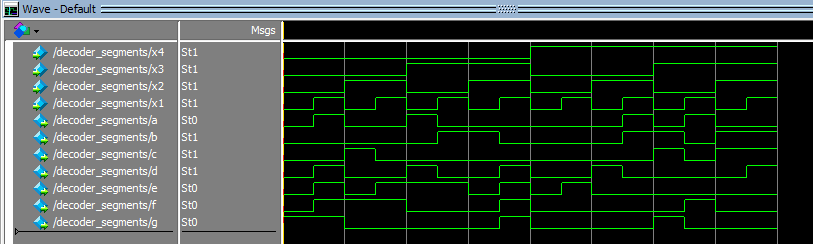
\includegraphics[width=\textwidth]{media/timediag.png}
        \caption{Часова діаграма семисегментного дешифратора}
    \end{figure}

    Усі значення вихідних сигналів сегментів збігаються зі значеннями в таблиці істинності, що свідчить про коректність синтезу дешифратора та можливість його подальшого використання.

    \begin{center} \textbf{\Large Висновок} \end{center}

    У ході виконання лабораторної роботи було розроблено дешифратор для семисегментного індикатора з активним рівнем логічного нуля. За заданим варіантом складено таблицю істинності для функцій керування сегментами $a, b, c, d, e, f, g$, після чого виконано їх мінімізацію за допомогою діаграм Вейча. Для функцій $a, b, c, d, e, f$ обрано мінімізовану КНФ, а для функції $g$ -- мінімізовану ДНФ, оскільки ці форми дали компактніші логічні вирази.

    На основі отриманих мінімізованих функцій дешифратор було описано мовою Verilog та перевірено за допомогою симуляції. Часова діаграма підтвердила, що вихідні сигнали відповідають таблиці істинності для всіх комбінацій входів $x_4, x_3, x_2, x_1$. Отже, синтезована схема працює коректно і може бути використана для керування семисегментним індикатором.

\end{document}